\documentclass{article}
\usepackage{amsmath,amssymb,amsthm,kotex,paralist,mathrsfs,url}

\newcounter{num}[section]
\newcommand{\defi}[1]
{\bigskip\noindent\refstepcounter{num}\textbf{정의 \arabic{section}. \arabic{num}) #1}\par}
\newcommand{\theo}[1]
{\bigskip\noindent\refstepcounter{num}\textbf{정리 \arabic{section}. \arabic{num}) #1}\par}
\newcommand{\axio}[1]

\begin{document}
\title{현빈 : 09 산술--기하 부등식, 코시--슈바르츠 부등식}
\author{}
\date{\today}
\maketitle

\section{산술--기하 부등식}
산술평균(Arithmetic Mean), 기하평균(Geometric Mean), 조화평균(Harmonic Mean) 사이의 관계를 나타내는 부등식이다.

\defi{산술평균, 기하평균, 조화평균}
양수 \(x_1\), \(x_2\), \(\cdots\), \(x_n\)에 대해, 산술평균 \(A\)는 
\[A=\frac{x_1+x_2+\cdots+x_n}n\]
이다.
또 기하평균 \(G\)는
\[G=\sqrt[n]{x_1\times x_2\times\cdots\times x_n}\]
이다.
마지막으로 조화평균 \(H\)는
\[\frac1H=\frac{\frac1{x_1}+\frac1{x_2}+\cdots+\frac1{x_n}}n\]
을 만족시키는 값이다.
즉
\[H=\frac n{\frac1{x_1}+\frac1{x_2}+\cdots+\frac1{x_n}}\]
이다.

\theo{}
정의 1.1에서 정의한 세 평균에 대해
\[A\ge G\ge H\]
가 성립한다.
이때 등호는 \(x_1=\cdots=x_n\)일 때 성립한다.

\begin{proof}
일반적인 경우의 증명은 수학적 귀납법(Mathematical Induction) 등을 통해 증명할 수 있다.
(cf. \url{http://en.wikipedia.org/wiki/Inequality_of_arithmetic_and_geometric_means})
여기서는 \(n=2\)일때, \(n=3\)일 때의 증명만 간단하게 소개한다.

(1) \(n=2\)\\
두 변량을 \(a\), \(b\)라고 할 때(\(a,b>0\))
\[A=\frac{a+b}2,\quad G=\sqrt{ab},\quad H=\frac{2ab}{a+b}\]
이다.
그러면
\begin{align*}
&A\ge G\\
\iff&a+b\le2\sqrt{ab}\\
\iff&(a+b)^2\ge 4ab\\
\iff&(a-b)^2\ge0
\end{align*}
이다.
이때, 등호는 \(a=b\)일 때 성립한다.
이는 증명과정에서 명백하다.
또
\begin{align*}
&G\ge H\\
\iff&1\ge\frac{2\sqrt{ab}}{a+b}\\
\iff&a+b\ge2\sqrt{ab}\\
\iff&A\ge G
\end{align*}
이다.
이때 등호는 \(a=b\)일 때 성립한다.

(2) \(n=3\)\\
세 변량을 \(a\), \(b\), \(c\)라고 할 때 (\(a,b,c>0\))
\[A=\frac{a+b+c}3,\quad G=\sqrt[3]{abc},\quad H=\frac{3abc}{ab+bc+ca}\]
이다.
\(x=\sqrt[3]a\), \(y=\sqrt[3]b\), \(z=\sqrt[3]c\)라고 하면
\begin{align*}
&A\ge G\\
\iff&a+b+c\ge3\sqrt[3]{abc}\\
\iff&x^3+y^3+z^3-3xyz\ge0\\
\iff&(x+y+z)(x^2+y^2+z^2-xy-yz-zx)
\end{align*}
이다.
이때, 등호는 \(a=b=c\)일 때 성립한다.
이는 증명과정에서 명백하다.

또
\begin{align*}
G\ge H\\
\iff&1\ge\frac{3(\sqrt[3]{abc})^2}{ab+bc+ca}\\
\iff&ab+bc+ca\ge3(\sqrt[3]{abc})^2
\end{align*}
인데 마지막 줄은 \(ab\), \(bc\), \(ca\)에 대해 \(A\ge G\)를 쓰면 얻어진다.
이때 등호는 \(ab=bc=ca\)일 때, 즉 \(a=b=c\)일 때, 성립한다.
\end{proof}

\section{코시-슈바르츠 부등식}
수학자 Augustin-Louis Cauchy(프랑스, 1821), Hermann Amandus Schwarz(독일, 1888)의 이름을 따서 명명한 중요한 부등식이다.
대개 두 사람의 이름만을 따서 Cauchy-Schwarz Inequality라고 부르지만 경우에 따라서는 Viktor Bunyakovsky(러시아, 1859)의 이름도 함께 붙여 Cauchy-Schwarz-Bunyakovsky Inequality라고 부르기도 한다.

여기에서는 단순히 \(n\)개의 변량에 관한 코시-슈바르츠 부등식을 다루지만, 일반적으로는 내적이 존재하는 벡터공간(vector space with inner product)에서 항상 성립한다.
적분가능한 실함수의 집합도 벡터공간을 이룬다는 점에서 적분에 관한 코시-슈바르츠 부등식도 성립하는데 역시 아주 중요한 부등식 중의 하나이다.

\theo{코시-슈바르츠 부등식}
\(x_1\), \(x_2\), \(\cdots\), \(x_n\), \(y_1\), \(y_2\), \(\cdots\), \(y_n\)이 실수이면 다음이 성립한다.
\[
({x_1}^2+\cdots+{x_n}^2)({y_1}^2+\cdots+{y_n}^2)\ge(x_1y_1+\cdots x_ny_n)^2
\]
이때 등호는 \(x_1=ky_1\), \(\cdots\) \(x_n=ky_n\)을 만족하는 실수 \(k\)가 존재할 때(혹은 그 반대일 때) 성립한다.
즉 \(x_1\), \(\cdots\), \(x_n\)이 0이 아니라고 하면
\[\frac{y_1}{x_1}=\cdots=\frac{y_n}{x_n}\]
일 때 등호가 성립한다.
\begin{proof}
산술-기하 부등식과 마찬가지로 일반적인 경우의 증명은 생략한다.

\(n=2\)이면 네 실수 \(a\), \(b\), \(x\), \(y\)에 대해
\[(a^2+b^2)(x^2+y^2)\ge(ax+by)^2\]
이 성립함을 보이면 된다;
\begin{align*}
&(a^2+b^2)(x^2+y^2)\ge(ax+by)^2\\
\iff&a^2x^2+a^2y^2+b^2x^2+b^2y^2\ge a^2x^2+2abxy+b^2y^2\\
\iff&(ay)^2-2(ay)(bx)+(bx)^2\\
\iff&(ay-bx)^2\ge0
\end{align*}
이때 등호는 \(ay=bx\)일 떄, 즉 \(a=kx\), \(b=ky\)를 만족시키는 실수 \(k\)가 존재할 때 성립한다.

\(n=3\)이면 여섯 개의 실수 \(a\), \(b\), \(c\), \(x\), \(y\), \(z\)에 대해
\[(a^2+b^2+c^2)(x^2+y^2+z^2)\ge(ax+by+cz)^2\]
\(n=2\)일 때와 마찬가지로 우변으로 이항하여 정리하면
\[(ay-bx)^2+(az-cx)^2+(bz-cy)^2\ge0\]
이 되어 성립한다.
이때 등호는 \(ay=bx\), \(az=cx\), \(bz=cy\)일 떄, 즉 \(a=kb\), \(x=ky\)를 만족시키는 실수 \(k\)가 존재할 때이다.
\end{proof}

--------------------- 예 제 ---------------------

28.
\(x>0\), \(y>0\), \(xy=1\)일 때, \(3x+2y\)의 최솟값을 구하여라.

\bigskip
29.
\(x>0\), \(y>0\)이고 \(3x+2y=16\)일 때, \(\sqrt{3x}+\sqrt{2y}\)의 최댓값을 구하여라.

\bigskip
30.
\(x>1\)일 때, \(4x+\frac1{x-1}\)의 최솟값을 구하여라.

\bigskip
31.
\(a>0\), \(b>0\)일 때, \((a+\frac1b)(b+\frac4a)\)의 최솟값을 구하여라.

\bigskip
32.
\(x\), \(y\), \(z\)가 실수일 때, 다음 물음에 답하여라.

\quad\:
(1) \(3x+4y=5\)일 때, \(x^2+y^2\)의 최솟값을 구하여라.

\quad\:
(2) \(x^2+y^2+z^2=14\)일 때, \(3x+2y+z\) 값의 범위를 구하여라.

\bigskip
34. 수직인 두 벽면 사이를 길이가 20m인 철망으로 막은 직각삼각형 모양의 닭장이 있다. 이 닭장의 넓이의 최댓값을 구하여라.
\begin{figure}[h]
\centering
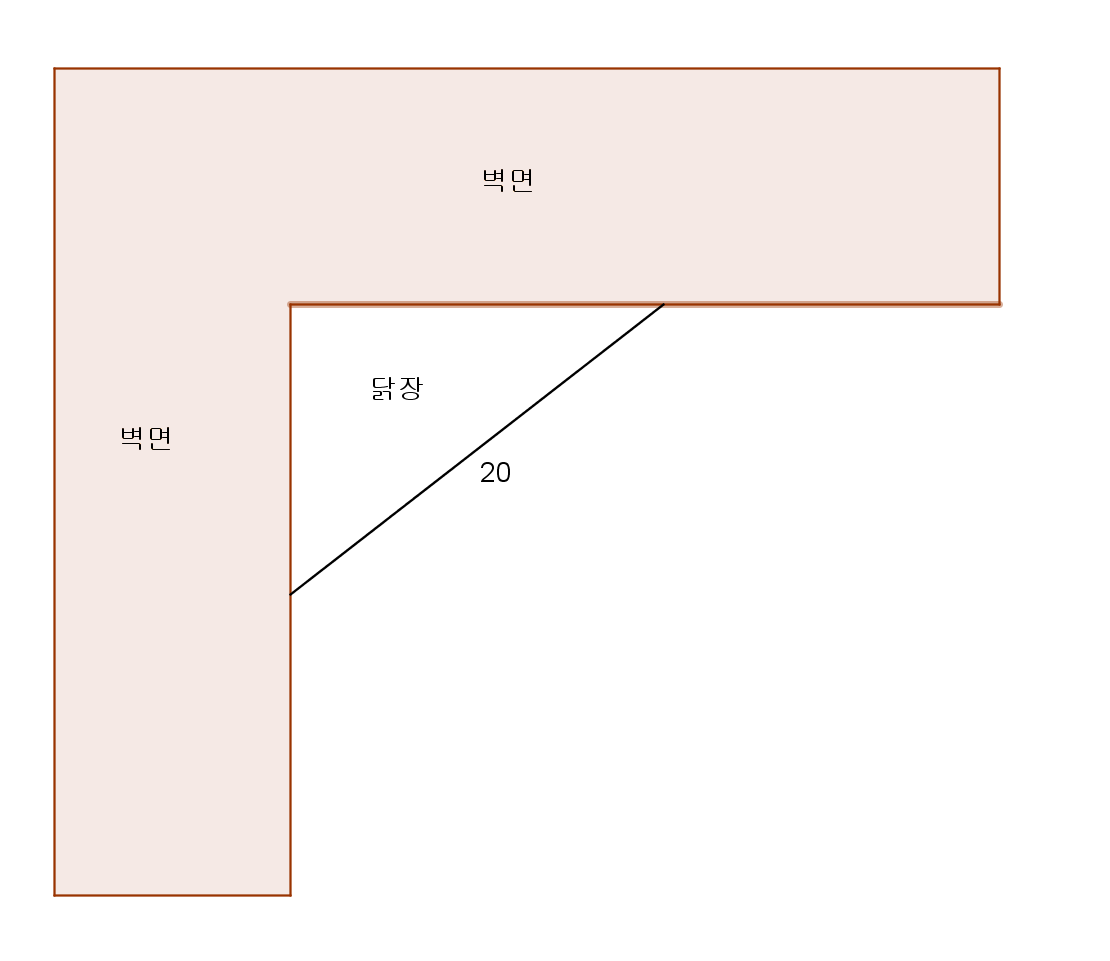
\includegraphics[width=0.5\textwidth]{34}
\end{figure}

--------------------- 연습 문제 ---------------------

83.
\(a>0\), \(b>0\), \(c>0\)일 때, 다음 부등식을 증명하여라.

\quad\:
(1) \((a+b)(\frac1a+\frac1b)\ge4\)

\quad\:
(2) \(a+b)(b+c)(c+a)\ge8abc\)

\bigskip
84.
\(a>0\), \(b>0\)이고 \(ab=3\)일 때, \(3a+4b\)의 최솟값을 구하여라.

\bigskip
85.
두 양수 \(a\), \(b\)가 \(9a^2+b^2=36\)을 만족시킬 때, \(ab\)의 최댓값을 구하여라.

\bigskip
86.
0이 아닌 두 실수 \(x\), \(y\)에 대하여 \(x^2+y^2=18\)일 때, \(xy\)의 최솟값을 구하여라.

\bigskip
87.
\(x>-2\)일 때, \(3x+5+\frac3{x+2}\)의 최솟값을 구하여라.

\bigskip
88.
\(a>0\), \(b>0\)일 때, \((3a+4b)(\frac3a+\frac1b)\)의 최솟값을 구하여라.

\bigskip
89.
실수 \(x\), \(y\)에 대하여 \(x^2+y^2=4\)일 때, \(4x+3y\)의 값의 범위를 구하여라.

\bigskip
90.
실수 \(a\), \(b\), \(x\), \(y\)에 대하여 \(a^2+b^2=2\), \(x^2+y^2=3\)일 때, \(ax+by\)의 최댓값을 구하여라.

\bigskip
91.
실수 \(a\), \(b\), \(c\)에 대하여 \(a^2+b^2+c^2=2\)일 때, \(a+2b+3c\)의 최솟값을 구하여라.

--------------------- 추가 문제 ---------------------

97.
다음 물음에 답하여라.

\quad\:
(1) \(x>0\), \(y>0\)일 때, \((2x+\frac1y)(\frac1x+8y)\)의 최솟값을 \(m\), 그 때의 \(xy\)값을 \(n\)이라 하자.
이 때 \(mn\)의 값을 구하여라.

\quad\:
(2) \(a\ge0\), \(b\ge0\)이고 \(a+b=5\)일 떄, \(\sqrt a+2\sqrt b\)의 최댓값을 구하여라.

\quad\:
(3) 실수 \(x\), \(y\)에 대하여 \(4x+3y=5\)일 때, \(x^2+y^2\)의 최솟값을 구하여라.

\bigskip
99.
다음 물음에 답하여라.

\quad\:
(2) 양수 \(x\)에 대하여 \(\frac{x^2+2x+2}{x}\)는 \(x=a\)에서 최솟값 \(b\)를 가질 때, \(-2a+b+3\)의 값을 구하여라.

\quad\:
(3) \(x>3\)일 때, \(3x-8+\frac1{x-3}\)의 최솟값을 \(a\), 그 때의 \(x\)의 값을 \(b\)라고 하자.
이때 \(6b-a\)의 값을 구하여라.

\bigskip
101.
\(a>0\), \(b>0\), \(c>0\)일 때, 다음 식의 최솟값을 구하여라.

\quad\:
(1) \(8a+\frac4{a^2}\)

\quad\:
(2) \((1+\frac{2b}a)(1+\frac cb)(1+\frac a{2c})\)

\quad\:
(3) \((a+b+c)(\frac1a+\frac1{b+c}\))

\bigskip
104.
실수 \(x\)에 대하여 \(x^2-x+\frac9{x^2-x+1}\)의 최솟값을 \(a\), 그때의 모든 \(x\)의 값의 합을 \(b\)라고 할 때, \(a+b\)의 값을 구하여라.
\end{document}